\everymath{\displaystyle}
\documentclass{beamer}
% \documentclass[handout]{beamer}

%\usepackage[pdftex]{color,graphicx}
\usepackage{amsmath,amssymb,amsfonts}

\mode<presentation>
{
  % \usetheme{Darmstadt}
  % \usetheme[hideothersubsections]{Hannover}
  % \usetheme[hideothersubsections]{Goettingen}
  \usetheme[hideothersubsections, right]{Berkeley}

  \usecolortheme{seahorse}
  % \usecolortheme{dolphin}
  \usecolortheme{rose}
  % \usecolortheme{orchid}

  \useinnertheme[shadow]{rounded}

  \setbeamercovered{transparent}
  % or whatever (possibly just delete it)
}

\mode<handout>{
  \setbeamercolor{background canvas}{bg=black!5}
  \usepackage{pgfpages}
  \pgfpagesuselayout{4 on 1}[a4paper,border shrink=5mm, landscape]
}

\usepackage[brazilian]{babel}
% or whatever

% \usepackage[latin1]{inputenc}
\usepackage[utf8]{inputenc}
% or whatever

\usepackage{times}
%\usepackage[T1]{fontenc}
% Or whatever. Note that the encoding and the font should match. If T1
% does not look nice, try deleting the line with the fontenc.


\title%[] % (optional, use only with long paper titles)
{Revisão bibliográfica e Resumo}

\subtitle
{Para que servem, tipos, e dicas} % (optional)

\author%[] % (optional, use only with lots of authors)
{Felipe Figueiredo}% \and S.~Another\inst{2}}
% - Use the \inst{?} command only if the authors have different
%   affiliation.

\institute[INTO] % (optional, but mostly needed)
{Instituto Nacional de Traumatologia e Ortopedia
}
  % \inst{1}%
  % Department of Computer Science\\
  % University of Somewhere
  % \and
  % \inst{2}%
  % Department of Theoretical Philosophy\\
  % University of Elsewhere}
% - Use the \inst command only if there are several affiliations.
% - Keep it simple, no one is interested in your street address.

\date%[] % (optional)
{}

% \subject{Talks}
% This is only inserted into the PDF information catalog. Can be left
% out. 



% If you have a file called "university-logo-filename.xxx", where xxx
% is a graphic format that can be processed by latex or pdflatex,
% resp., then you can add a logo as follows:

\pgfdeclareimage[height=1.6cm]{university-logo}{../logo}
\logo{\pgfuseimage{university-logo}}



% Delete this, if you do not want the table of contents to pop up at
% the beginning of each subsection:
\AtBeginSubsection[]
%\AtBeginSection[]
{
  \begin{frame}<beamer>{Sumário}
    \tableofcontents[currentsection,currentsubsection]
  \end{frame}
}


% If you wish to uncover everything in a step-wise fashion, uncomment
% the following command: 

% \beamerdefaultoverlayspecification{<+->}


\begin{document}

\begin{frame}
  \titlepage
\end{frame}

\begin{frame}{Sumário}
  \tableofcontents
  % You might wish to add the option [pausesections]
\end{frame}


%% Template
% \section{}

% \subsection{}

% \begin{frame}{}
%   \begin{itemize}
%   \item 
%   \end{itemize}
% \end{frame}

% \begin{frame}
%   \begin{columns}
%     \begin{column}{5cm}
%     \end{column}
%     \begin{column}{5cm}
%     \end{column}
%   \end{columns}
% \end{frame}

% \begin{frame}{}
%   \includegraphics[height=0.4\textheight]{file1}
%   \includegraphics[height=0.4\textheight]{file2}
%   \includegraphics[height=0.4\textheight]{file3}
%   \begin{figure}
%     \caption{}
%   \end{figure}
% \end{frame}

% \begin{frame}{}
%   \begin{definition}
%   \end{definition}
%   \begin{example}
%   \end{example}
%   \begin{block}{Exercício}
%   \end{block}
% \end{frame}

\section{Discussão da aula passada}

% \subsection{Discussão da aula passada}

\begin{frame}{Discussão da aula passada}
  \begin{block}{}
    Discussão da leitura obrigatória da aula passada
  \end{block}
\end{frame}

\section{Revisão da literatura}

\subsection{Revisão da literatura}

\begin{frame}{Revisão bibliográfica x Introdução}
  \begin{block}{}
    \footnotesize
    A Introdução do projeto ou dissertação tem algumas semelhanças com
    um artigo de Revisão Bibliográfica.

    \bigskip

    Vamos analisar os principais aspectos de uma revisão que servem
    para ambos os casos.
  \end{block}
\end{frame}

\begin{frame}
  \begin{block}{Atenção}
    \begin{center}
      Não há lugar num trabalho acadêmico para alegações do tipo {\em ``é sabido que''}!
    \end{center}
  \end{block}
\end{frame}

\begin{frame}{Revisão bibliográfica x Introdução}
  \begin{center}
    \footnotesize
    A introdução do trab. acad. é uma {\bf revisão da literatura}...

    \bigskip
    \normalsize
    \visible<2->{... e \alert{\bf cada} afirmação ou alegação feita deve ser

      \alert{embasada com referências}}
  \end{center}
\end{frame}

\begin{frame}{Como se manter atualizado na literatura?}
  \begin{center}
    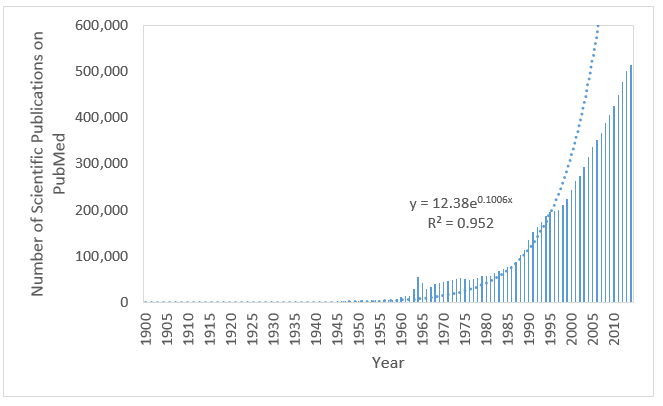
\includegraphics[width=1.2\textwidth]{Revisao_resumo/pubs-year}
  \end{center}
\end{frame}

\begin{frame}{Quando fazer uma revisão?}
  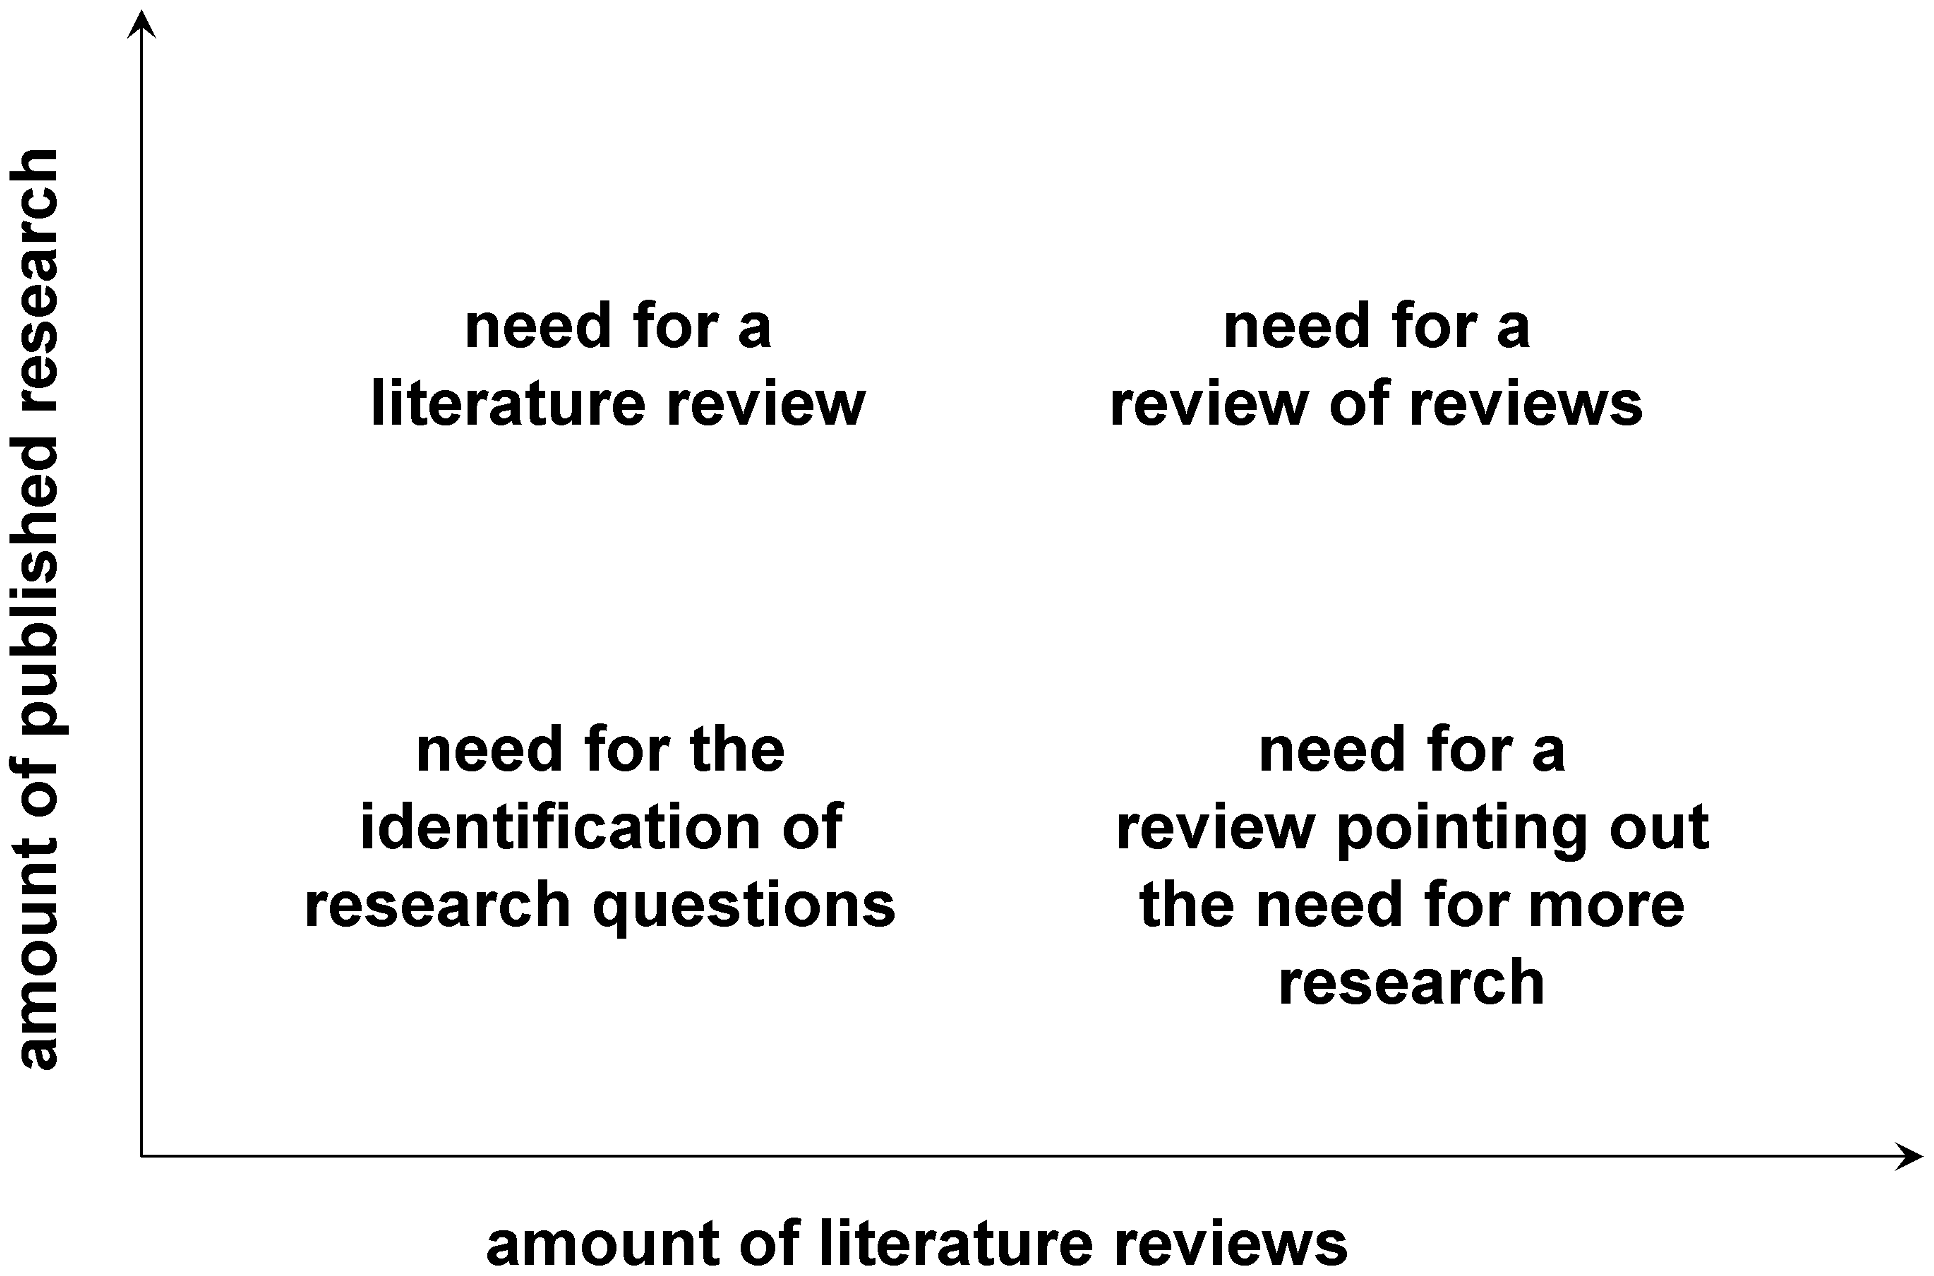
\includegraphics[height=0.8\textheight]{Revisao_resumo/10_dicas_revisao}

  \vfill
  \scriptsize
  \hfill Fonte: \href{https://doi.org/10.1371/journal.pcbi.1003149}{Pautasso, 2013}
\end{frame}

\begin{frame}{Objetivos da Revisão}
  \begin{itemize}
    \footnotesize
  \item Discutir e sintetizar resultados sobre um assunto
    \bigskip
  \item Sintetizar obtidos de fontes primárias
    \bigskip
  \item Oferecer uma nova perspectiva para a área
  \end{itemize}

  \vfill
  \scriptsize
  \hfill Fonte: \href{https://writing.colostate.edu/guides/guide.cfm?guideid=79}
  {\tiny Writing@CSU Guide -- Review Essays for the Biological sciences}
\end{frame}

\subsection{Tipos}

\begin{frame}{Tipos de Revisão da literatura}
  \begin{itemize}
    \footnotesize
  \item Narrativa (overview)
    \bigskip
  \item Sistemática
    \begin{itemize}
      \scriptsize
      \medskip
    \item sem meta-análise
      \smallskip
    \item com meta-análise
    \end{itemize}
  \end{itemize}
\end{frame}

\subsubsection[Narrativa]{Revisão narrativa}

\begin{frame}{Revisão narrativa}
  \begin{itemize}
    \scriptsize
  \item Estado da arte
    \bigskip
  \item Comparação entre perspectivas
    \bigskip
  \item Síntese de duas áreas
    \bigskip
  \item Formulação de modelo teórico
    \bigskip
  \item Histórica
  \end{itemize}

  \vfill
  \scriptsize
  \hfill Fonte: \href{https://writing.colostate.edu/guides/guide.cfm?guideid=79}
  {\tiny Writing@CSU Guide -- Review Essays for the Biological sciences}
\end{frame}

\begin{frame}{Considerações}
  \begin{itemize}
    \footnotesize
  \item Foco estreito
    \bigskip
  \item Fontes primárias
    \bigskip
  \item Referencie as fontes
    \bigskip
  \item Poucas citações diretas
  \end{itemize}

  \vfill
  \scriptsize
  \hfill Fonte: \href{https://writing.colostate.edu/guides/guide.cfm?guideid=79}
  {\tiny Writing@CSU Guide -- Review Essays for the Biological sciences}
\end{frame}

\subsubsection[Sistemática]{Revisão sistemática}

\begin{frame}{Revisão sistemática}
  \begin{block}{Definição}
    \footnotesize
    ... agrega toda a evidência empírica que atende a critérios de elegibilidade pré-definidos para responder a um problema de pesquisa específico.
  \end{block}

  \vfill
  \scriptsize
  \hfill Fonte: \href{https://doi.org/10.1371/journal.pmed.1000100}
  {\tiny PRISMA Explanation \& Elaboration (2009)}
\end{frame}

\begin{frame}{PRISMA statement}
  \begin{center}
    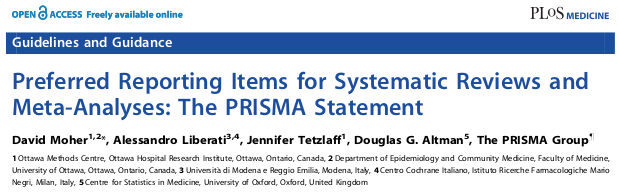
\includegraphics[width=\textwidth]{Revisao_resumo/PRISMA-statement}
  \end{center}

  \vfill
  \scriptsize
  \hfill Fonte: \href{https://doi.org/10.1371/journal.pmed.1000097}
  {\tiny PRISMA statement (2009)}
\end{frame}

\begin{frame}{PRISMA checklist -- 27 itens no total}
  \begin{center}
    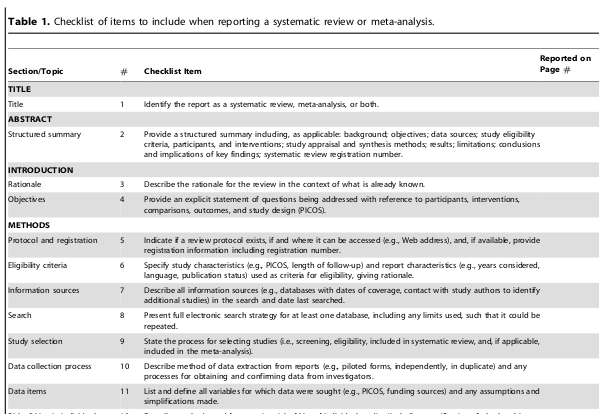
\includegraphics[height=.8\textheight]{Revisao_resumo/PRISMA-checklist}
  \end{center}

  \vfill
  \scriptsize
  \hfill \href{http://www.prisma-statement.org/}
  {\tiny Disponível em PRISMA-statement.org (DOC)}
\end{frame}

\begin{frame}{PRISMA}
  \begin{center}
    E como preencher os itens necessários ao relatório?
  \end{center}
\end{frame}

\begin{frame}{PRISMA -- Explicação \& Elaboração}
  \begin{center}
    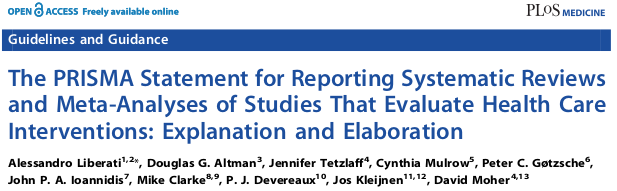
\includegraphics[width=\textwidth]{Revisao_resumo/PRISMA-EE}
  \end{center}

  \vfill
  \scriptsize
  \hfill Fonte: \href{https://doi.org/10.1371/journal.pmed.1000100}
  {\tiny PRISMA Explanation \& Elaboration (2009)}
\end{frame}

\begin{frame}{PRISMA -- flow diagram}
  \begin{center}
    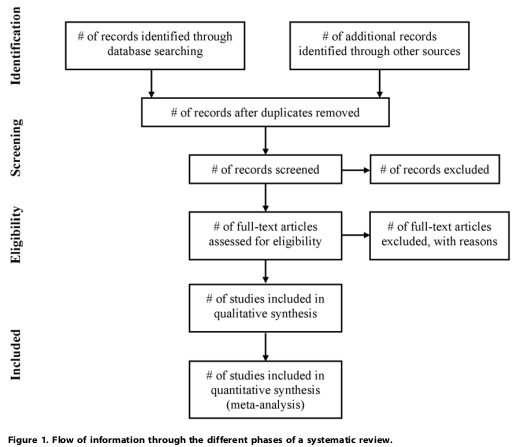
\includegraphics[height=.8\textheight]{Revisao_resumo/PRISMA-flow}
  \end{center}

  \vfill
  \scriptsize
  \hfill \href{http://www.prisma-statement.org/}
  {\tiny Disponível em PRISMA-statement.org (DOC)}
\end{frame}

\begin{frame}{\tiny \bf Prevalence of chronic low back pain: systematic review}
  \begin{exampleblock}{Exemplo}
    \tiny
{\bf OBJECTIVE}
To estimate worldwide prevalence of chronic low back pain according to age and sex.

{\bf METHODS}
We consulted Medline (PubMed), LILACS and EMBASE electronic databases.
The search strategy used the following descriptors and combinations: back pain, prevalence, musculoskeletal diseases, chronic musculoskeletal pain, rheumatic, low back pain, musculoskeletal disorders and chronic low back pain.
We selected cross-sectional population-based or cohort studies that assessed chronic low back pain as an outcome.
We also assessed the quality of the selected studies as well as the chronic low back pain prevalence according to age and sex.

{\bf RESULTS}
The review included 28 studies.
  Based on our qualitative evaluation, around one third of the studies had low scores, mainly due to high non-response rates.
Chronic low back pain prevalence was 4.2\% in individuals aged between 24 and 39 years old and 19.6\% in those aged between 20 and 59.
\alert{\bf \scriptsize Of nine studies with individuals aged 18 and above, six reported chronic low back pain between 3.9\% and 10.2\% and three, prevalence between 13.1\% and 20.3\%.}
In the Brazilian older population, chronic low back pain prevalence was 25.4\%.

{\bf CONCLUSIONS}
Chronic low back pain prevalence increases linearly from the third decade of life on, until the 60 years of age, being more prevalent in women. Methodological approaches aiming to reduce high heterogeneity in case definitions of chronic low back pain are essential to consistency and comparative analysis between studies. A standard chronic low back pain definition should include the precise description of the anatomical area, pain duration and limitation level.
  \end{exampleblock}

  \vfill
  \scriptsize
  \hfill Fonte: \href{https://doi.org/10.1590/S0034-8910.2015049005874}
  {Meucci, Fassa e Faria, 2015}
\end{frame}

\begin{frame}{\tiny \bf Could low grade bacterial infection contribute to low back pain? A systematic review}
  \begin{exampleblock}{Exemplo}
    \tiny
{\bf Background:}
Recently, there has been both immense interest and controversy regarding a randomised, controlled
trial which showed antibiotics to be effective in the treatment of chronic low back pain (disc herniation with Modic
Type 1 change). While this research has the potential to result in a paradigm shift in the treatment of low back
pain, several questions remain unanswered. This systematic review aims to address these questions by examining
the role of bacteria in low back pain and the relationship between bacteria and Modic change.

{\bf Methods:}
We conducted electronic searches of MEDLINE and EMBASE and included studies that examined the
relationship between bacteria and back pain or Modic change. Studies were rated based on their methodological
quality, a best-evidence synthesis was used to summarise the results, and Bradford Hill’s criteria were used to assess
the evidence for causation.

{\bf Results:}
\alert{\bf \scriptsize Eleven studies were identified.
The median (range) age and percentage of female participants was 44.7 (41–46.4) years and 41.5\% (27–59\%), respectively, and in 7 of the 11 studies participants were diagnosed with disc herniation.}
Nine studies examined the presence of bacteria in spinal disc material and all identified bacteria, with
the pooled estimate of the proportion with positive samples being 34\%.
Propionibacterium acnes was the most
prevalent bacteria, being present in 7 of the 9 studies, with median (minimum, maximum) 45.0\% (0–86.0) of
samples positive. The best evidence synthesis found moderate evidence for a relationship between the presence of
bacteria and both low back pain with disc herniation and Modic Type 1 change with disc herniation. There was
modest evidence for a cause-effect relationship.

{\bf Conclusions:} We found that bacteria were common in the spinal disc material of people undergoing spinal
surgery. There was moderate evidence for a relationship between the presence of bacteria and both low back pain
with disc herniation and Modic Type 1 change associated with disc herniation and modest evidence for causation.
However, further work is needed to determine whether these organisms are a result of contamination or represent
low grade infection of the spine which contributes to chronic low back pain.
  \end{exampleblock}

  \vfill
  \scriptsize
  \hfill Fonte: \href{https://doi.org/10.1186/s12916-015-0267-x}
  {Urquhart et al, 2015}
\end{frame}

\begin{frame}{\footnotesize Cochrane Library -- evidências para a prática clínica}
  \begin{block}{55 grupos temáticos especializados}
    \begin{center}
      \begin{itemize}
        \tiny
      \item Anaesthesia
      \item Back and Neck
      \item Bone, Joint and Muscle Trauma
      \item Cystic Fibrosis and Genetic Disorders
      \item Emergency and Critical Care
      \item Injuries
      \item Metabolic and Endocrine Disorders
      \item Methodology
      \item Movement Disorders
      \item Musculoskeletal
      \item Neuromuscular
      \item Public Health
      \item ...
      \end{itemize}
    \end{center}
  \end{block}

  \vfill
  \scriptsize
  \hfill\href{https://www.cochranelibrary.com/about/cochrane-review-groups}{Cochrane Review Groups}
\end{frame}

\subsubsection[Meta-análise]{Revisão sistemática com meta-análise}

\begin{frame}{Meta-análises}
  \begin{block}{Definição}
    \footnotesize
    ... o uso de técnicas estatísticas para integrar e sumarizar os resultados dos estudo incluídos.
  \end{block}

  \vfill
  \scriptsize
  \hfill Fonte: \href{https://doi.org/10.1371/journal.pmed.1000100}
  {\tiny PRISMA Explanation \& Elaboration}
\end{frame}

\begin{frame}{\tiny \bf Systematic Literature Review of Imaging Features of Spinal Degeneration in Asymptomatic Populations}
  \begin{exampleblock}{Exemplo}
    \tiny
    {\bf BACKGROUND AND PURPOSE:} Degenerative changes are commonly found in spine imaging but often occur in pain-free individuals as well as those with back pain.
    \alert{\bf \scriptsize We sought to estimate} the prevalence, by age, of common degenerative spine conditions by performing a systematic review studying the prevalence of spine degeneration on imaging in asymptomatic individuals.

    {\bf MATERIALS AND METHODS:} We performed a systematic review of articles reporting the prevalence of imaging findings (CT or MR imaging) in asymptomatic individuals from published English literature through April 2014.
    Two reviewers evaluated each manuscript.
    We selected age groupings by decade (20, 30, 40, 50, 60, 70, 80 years), determining age-specific prevalence estimates.
    For each imaging finding, \alert{\bf \scriptsize we fit a generalized linear mixed-effects model for the} age-specific prevalence estimate clustering in the study, adjusting for the midpoint of the reported age interval.

    {\bf RESULTS:} Thirty-three articles reporting imaging findings for 3110 asymptomatic individuals met our study inclusion criteria.
    The prevalence of disk degeneration in asymptomatic individuals increased from 37\% of 20-year-old individuals to 96\% of 80-year-old individuals.
    Disk bulge prevalence increased from 30\% of those 20 years of age to 84\% of those 80 years of age. Disk protrusion prevalence increased from 29\% of those 20 years of age to 43\% of those 80 years of age.
    The prevalence of annular fissure increased from 19\% of those 20 years of age to 29\% of those 80 years of age.

{\bf CONCLUSIONS:} Imaging findings of spine degeneration are present in high proportions of asymptomatic individuals, increasing with age.
Many imaging-based degenerative features are likely part of normal aging and unassociated with pain.
These imaging findings must be interpreted in the context of the patient’s clinical condition.
  \end{exampleblock}
  \vfill
  \scriptsize
  \hfill Fonte: \href{http://dx.doi.org/10.3174/ajnr.A4173}
  {\tiny Brinjikji et al, 2015}
\end{frame}

\subsection{Dicas}

\begin{frame}{10 dicas para um artigo de revisão}
  \begin{enumerate}
    \scriptsize
  \item Definir tópico e público alvo
    \smallskip
  \item Pesquisa abrangente na literatura
    \smallskip
  \item Faça anotações enquanto lê
    \smallskip
  \item Escolha o tipo de revisão
    \smallskip
  \item Texto focado mas de interesse abrangente
    \smallskip
  \item Seja crítico e consistente
    \smallskip
  \item Estrutura lógica
    \smallskip
  \item Peça feedback
    \smallskip
  \item Inclua suas publicações, mas seja objetivo
    \smallskip
  \item Seja atual, mas não esqueça os estudos ``clássicos''
  \end{enumerate}

  \vfill
  \scriptsize
  \hfill Fonte: \href{https://doi.org/10.1371/journal.pcbi.1003149}{Pautasso, 2013}
\end{frame}

\section{Resumo}

\subsection{Resumo}

\begin{frame}{Definição}
  \begin{itemize}
    \footnotesize
  \item Mostra os aspectos principais do trabalho ou projeto
    \bigskip
  \item linguagem técnica, sucinto
    \bigskip
  \item curto
  \end{itemize}
\end{frame}

\begin{frame}{Objetivos do resumo}
  \begin{itemize}
    \footnotesize
  \item Ajudar o leitor a decidir se ele deve ler o texto completo
    \bigskip

%O leitor vai usar o abstract de artigos quando for fazer o levantamente bibliográfico.

  \item Ajudar o leitor a lembrar fatos importantes de um assunto
    \bigskip

%Depois de ler vários artigos, pode ser difícil para o leitor se lembrar onde uma certa informação ou fato foi obtido, para fins de citação

  \item Ajudar o leitor a entender um texto difícil (pré-leitura
    sumária)
    \bigskip

  \item Indexar artigos para fácil localização e referência
    \bigskip

  \item Permitir que supervisores se mantenham atualizados na produção
    do lab
  \end{itemize}
\end{frame}

\subsection{Tipos}

\begin{frame}{Tipos de resumo}
  \begin{itemize}
    \footnotesize
  \item Resumo descritivo
    \bigskip
    \bigskip
  \item Resumo estruturado (informativo)
  \end{itemize}

  \vfill
  \scriptsize
  \hfill Fonte: \href{https://writing.colostate.edu/guides/guide.cfm?guideid=59}{Writing@CSU Guide -- Abstracts}
\end{frame}

\subsubsection[Descritivo]{Resumo descritivo}

\begin{frame}{Resumo descritivo}
  \begin{itemize}
    \footnotesize
  \item Descreve os principais tópicos do texto
    \bigskip
  \item ``sumário em forma de parágrafo''
    \bigskip
  \item não substitui a leitura do texto
  \end{itemize}
\end{frame}

\begin{frame}{Resumo descritivo}
  \begin{exampleblock}{Exemplo}
    \scriptsize
    We continue to document all major climatic variables in the
    uplands and floodplains at Bonanza Creek. In addition, we have
    documented the successional changes in microclimate in 9
    successional upland and floodplain stands at Bonanza Creek (BNZ)
    and in four elevational locations at Caribou-Poker Creek
    (CPCRW). A sun photometer is operated cooperatively with NASA to
    estimate high-latitude atmospheric extinction coefficients for
    remote-sensing images. Electronic data are collected monthly and
    loaded into a database which produces monthly summaries.  (...)
  \end{exampleblock}

  \vfill
  \tiny
  \hfill ``Bonanza Creek LTER [Long Term Ecological Research] 1997 Annual
  Progress Report''
\end{frame}

\subsubsection[Estruturado]{Resumo estruturado}

\begin{frame}{Resumo estruturado}
  \begin{itemize}
    \footnotesize
  \item Inclui os detalhes essenciais do texto
    \bigskip
  \item É suficiente para a decisão de ler ou não o texto completo
    \bigskip
  \item Pode ser usado para mapear informações, fatos e dados
    \bigskip
  \item Mais usado para artigos experimentais
  \end{itemize}
\end{frame}

\begin{frame}{Resumo estruturado}
  Componentes típicos do resumo estruturado
  \begin{itemize}
    \footnotesize
  \item Contexto e/ou motivação
    \bigskip
  \item Objetivo, apresentação do problema
    \bigskip
  \item Metodologia (para trabalhos experimentais)
    \bigskip
  \item Principais resultados e descobertas
    \bigskip
  \item Principais conclusões
  \end{itemize}
\end{frame}

\begin{frame}{Resumo estruturado}
  \begin{exampleblock}{Exemplo}
    \scriptsize
    Research reported by Daly, Miller, and their colleagues suggests
    that writing apprehension is related to a number of factors we do
    not yet fully understand. This study suggests that included among
    those factors should be the belief that writing ability is a
    gift. Giftedness, as it is referred to in the study, is roughly
    equivalent to the Romantic notion of original genius. Results from
    a survey of 247 postsecondary students enrolled in introductory
    writing courses at two institutions indicate that higher levels of
    belief in giftedness are correlated with higher levels of writing
    apprehension, (...) 
  \end{exampleblock}
  % ``Palmquist, M., \& Young, R. (1992). The Notion of Giftedness and
  % Student Expectations About Writing. Written Communication, 9(1),
  % 137-168.''

  \vfill
  \scriptsize
  \hfill \href{https://doi.org/10.1177/0741088392009001004}{Palmquist e Young, 1992}
\end{frame}

\begin{frame}{Resumo estruturado}
  \begin{exampleblock}{Contexto, motivação}
    \scriptsize
    \alert{Research reported by Daly, Miller, and their colleagues
      suggests that writing apprehension is related to a number of
      factors we do not yet fully understand. This study suggests that
      included among those factors should be the belief that writing
      ability is a gift. Giftedness, as it is referred to in the
      study, is roughly equivalent to the Romantic notion of original
      genius.} Results from a survey of 247 postsecondary students
    enrolled in introductory writing courses at two institutions
    indicate that higher levels of belief in giftedness are correlated
    with higher levels of writing apprehension, (...)
  \end{exampleblock}

  \vfill
  \scriptsize
  \hfill \href{https://doi.org/10.1177/0741088392009001004}{Palmquist e Young, 1992}
\end{frame}

\begin{frame}{Resumo estruturado}
  \begin{exampleblock}{Metodologia}
    \scriptsize
    Research reported by Daly, Miller, and their colleagues suggests
    that writing apprehension is related to a number of factors we do
    not yet fully understand. This study suggests that included among
    those factors should be the belief that writing ability is a
    gift. Giftedness, as it is referred to in the study, is roughly
    equivalent to the Romantic notion of original genius. Results from
    \alert{a survey of 247 postsecondary students enrolled in
      introductory writing courses at two institutions} indicate that
    higher levels of belief in giftedness are correlated with higher
    levels of writing apprehension, (...)
  \end{exampleblock}

  \vfill
  \scriptsize
  \hfill \href{https://doi.org/10.1177/0741088392009001004}{Palmquist e Young, 1992}
\end{frame}

\begin{frame}{Resumo estruturado}
  \begin{exampleblock}{Resultados}
    \scriptsize
    Research reported by Daly, Miller, and their colleagues suggests
    that writing apprehension is related to a number of factors we do
    not yet fully understand. This study suggests that included among
    those factors should be the belief that writing ability is a
    gift. Giftedness, as it is referred to in the study, is roughly
    equivalent to the Romantic notion of original
    genius. \alert{Results} from a survey of 247 postsecondary
    students enrolled in introductory writing courses at two
    institutions \alert{indicate that higher levels of belief in
      giftedness are correlated with higher levels of writing
      apprehension,} (...)
  \end{exampleblock}

  \vfill
  \scriptsize
  \hfill \href{https://doi.org/10.1177/0741088392009001004}{Palmquist e Young, 1992}
\end{frame}

\section{Aprofundamento}

\subsection{Aprofundamento}

\begin{frame}{Aprofundamento}
  \begin{block}{Leitura obrigatória}
    \begin{itemize}
      \footnotesize
    \item \href{https://doi.org/10.1371/journal.pmed.1000100}
      {PRISMA Explanation \& Elaboration (2009) -- {\tiny guia}}
      \begin{itemize}
        \tiny
      \item {\bf Itens: 1, 2, 3, 4, 6, 7, 8, 9, 11, 17, 18, 20, 25 e 26.}
      \end{itemize}
      \smallskip
    \item {\footnotesize \href{https://doi.org/10.1371/journal.pmed.1000097}
        {PRISMA statement (2009) -- {\tiny história e contexto do problema resolvido pelo guia}}}
    \end{itemize}
  \end{block}
  \begin{block}{Leitura recomendada}
    \begin{itemize}
      \tiny
    \item
      \href{https://writing.colostate.edu/guides/guide.cfm?guideid=79}{Writing@CSU Guide -- Review Essays for the Biological sciences}
    \item \href{https://writing.colostate.edu/guides/guide.cfm?guideid=59}{Writing@CSU Guide -- Abstracts}
    \item \href{https://doi.org/10.1371/journal.pcbi.1003149}
      {PAUTASSO, Marco. Ten simple rules for writing a literature review. {\bf PLOS Computational Biology}, v. 9, n. 7, 2013.}
    \end{itemize}
    \begin{itemize}
      \tiny
    \item \url{http://metodologia.org/}
    \item Seções do livro texto: {\bf 4.7, 8.1.9}
    \end{itemize}
  \end{block}
\end{frame}

\end{document}
